\begin{pa} \label{PA:9.5}
We are familiar with equations of lines in the plane in the form $y = mx+b$, where $m$ is the slope of the line and $(0,b)$ is the $y$-intercept. In this activity, we explore a more flexible way of representing lines that we can use not only in the plane, but in higher dimensions as well.

To begin, consider the line through the point $(2,-1)$ with slope $\frac{2}{3}$.

\begin{figure}[ht]
  \begin{center}
    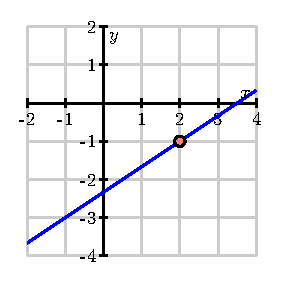
\includegraphics{fig_9_5_PA1.eps}
  \end{center}
\end{figure}
    \ba
      \item Suppose we increase $x$ by 1 from the point $(2,-1)$. How does the $y$-value change? What is the point on the line with $x$-coordinate $3$?

        \item Suppose we decrease $x$ by 3.25 from the point $(2,-1)$. How does the $y$-value change? What is the point on the line with $x$-coordinate $-1.25$?

        \item Now, suppose we increase $x$ by some arbitrary value $3t$ from the point $(2,-1)$. How does the $y$-value change? What is the point on the line with $x$-coordinate $2+3t$?


        \item Observe that the slope of the line is related to any vector whose $y$-component divided by the $x$-component is the slope of the line. For the line in this exercise, we might use the vector $\langle 3,2 \rangle$, which describes the direction of the line. Explain why the terminal points of the vectors $\vr(t)$, where
             \[\vr(t) = \langle 2,-1 \rangle + \langle 3,2 \rangle t, \]
             trace out the graph of the line through the point $(2,-1)$ with slope $\frac{2}{3}$.


    \item Now we extend this vector approach to $\R^3$ and consider a second example. Let $\mathcal{L}$ be the line in $\R^3$ through the point $(1,0,2)$ in the direction of the vector $\langle 2, -1, 4 \rangle$.

  Find the coordinates of three distinct points on line $\mathcal{L}$. Explain your thinking.


        \item Find a vector in form
        $$\vr(t) = \langle x_0, y_0, z_0 \rangle + \langle a,b,c \rangle t$$ whose terminal points trace out the line $\mathcal{L}$ that is described in (e).  That is, you should be able to locate any point on the line by determining a corresponding value of $t$.
        

    \ea

\end{pa} 



\begin{activitySolution}
    \ba
      \item The slope tells us how the $y$ values change for every unit increase in $x$. So if $x$ increases by 1 from the point $(2,-1)$, the $y$ value increases by $\frac{2}{3}$ to $-\frac{1}{3}$. The point on the line with $x$-coordinate $3$ is then $\left(3,-\frac{1}{3}\right)$.

        \item If $x$ changes by an amount $\Delta x$, then the corresponding change in $y$ is $\frac{\Delta y}{\Delta x} \Delta x$, where $\frac{\Delta y}{\Delta x}$ is the slope of the line. So if $x$ decreases by 3.25 from the point $(2,-1)$, then $y$ changes by ${\frac{2}{3}(-3.25) = -\frac{13}{6}}$. The corresponding point on the line is $\left(-1.25, -\frac{19}{6}\right)$.


        \item If $x$ changes by an amount $3t$, then the corresponding change in $y$ is $\frac{2}{3}(3t) = 2t$. So the new point on the line is ${(x,y) = (2+3t, -1+2t)}$.


        \item We saw in the previous part that an arbitrary point on this line has the form $(2+3t, -1+2t)$. If we think of these points as the terminal points of vectors $\vr(t)$, then we have
\[\vr(t) = \langle 2+3t, -1+2t \rangle =\langle 2,-1 \rangle + \langle 3,2 \rangle t.\]
So the terminal points of the vectors $\vr(t)$ trace out the graph of the line through the point $(2,-1)$ with slope $\frac{2}{3}$.


    \item The point $(1,0,2)$ is given as one point on the line. If we start at the point $(1,0,2)$ and move along the line one step in the direction of the vector $\langle 2, -1, 4 \rangle$, we will arrive at the point
 \[(1+2, 0+(-1), 2+4) = (3,-1,6).\]
Similarly, if we move two steps in the direction of the vector $\langle 2, -1, 4 \rangle$, we will arrive at the point
\[(1+4, 0+(-2), 2+8) = (5,-2,10).\]


        \item Starting at the point $(1,0,2)$ and moving along the line $t$ steps in the direction of the vector $\langle 2, -1, 4 \rangle$, we will arrive at the point
\[(1+2t, 0+(-t), 2+4t).\]
If we consider these points as the terminal points of vectors, we can describe the line as the set of terminal points of the vectors
\[\vr(t) = \langle 1,0,2 \rangle + \langle 2,-1,4\rangle t.\]


    \ea


\end{activitySolution}

\afterpa 